\documentclass[catalan, a4paper, nobib]{tufte-handout}

% encoding
\usepackage[utf8]{inputenc}
\usepackage[T1]{fontenc}
\usepackage{lmodern}
\usepackage{babel}

\frenchspacing
\usepackage[style=spanish]{csquotes}
\MakeAutoQuote{«}{»}

\usepackage{booktabs}
\usepackage{circuitikz}
\usepackage{siunitx}
\usepackage{amsmath}

\graphicspath{
    {fotos/}
}

% hyperlink setup / metadata
\usepackage{hyperref}
\AfterPreamble{\hypersetup{
  %%pdfauthor={},
  %%pdftitle={},
  %%pdfsubject={},
}}

\sisetup{per-mode = symbol}

% document metadata
\author{Sofija Starcevic i Víctor Méndez}
\title{FISE: Pràctica 3}
\date{19-2-2024}

\begin{document}

\maketitle

\part{Primera sessió}
\section{1. Resposta temporal}
\newthought{Qüestió 1.1} Veure la figura \ref{fig:q1}. El guany és $G=1$ i el desfasament és de \ang{180}.
\begin{figure}[h]
    \begin{center}
        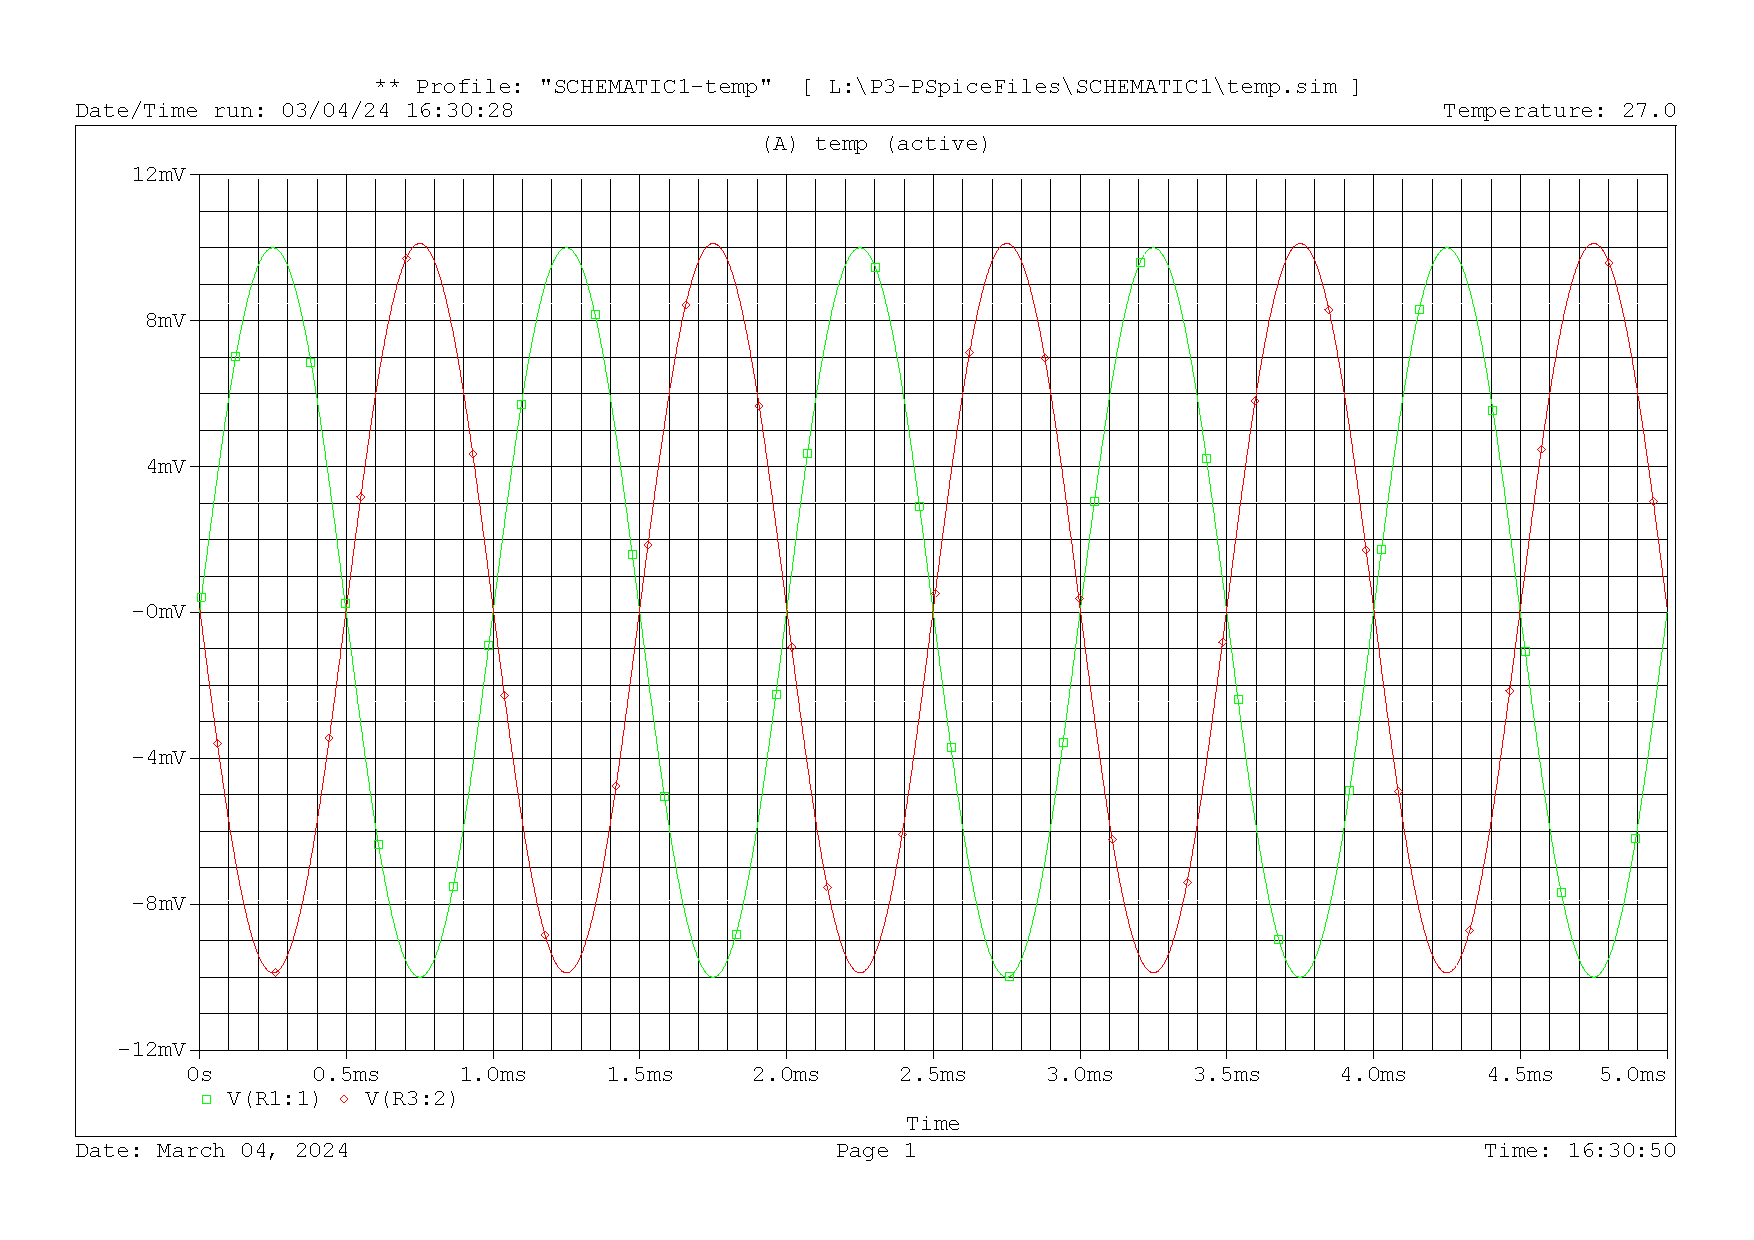
\includegraphics[width=\linewidth]{q1.pdf}
    \end{center}
    \caption{Entrada i sortida de l'inversor}
    \label{fig:q1}
\end{figure}

\newthought{Qüestió 1.2} Veure la figura \ref{fig:q2}. Les tensions son del ordre de \unit{\micro\volt}, son bastant negligibles. És força valid aplicar curtcircuit virtual.
\begin{figure}[h]
    \begin{center}
        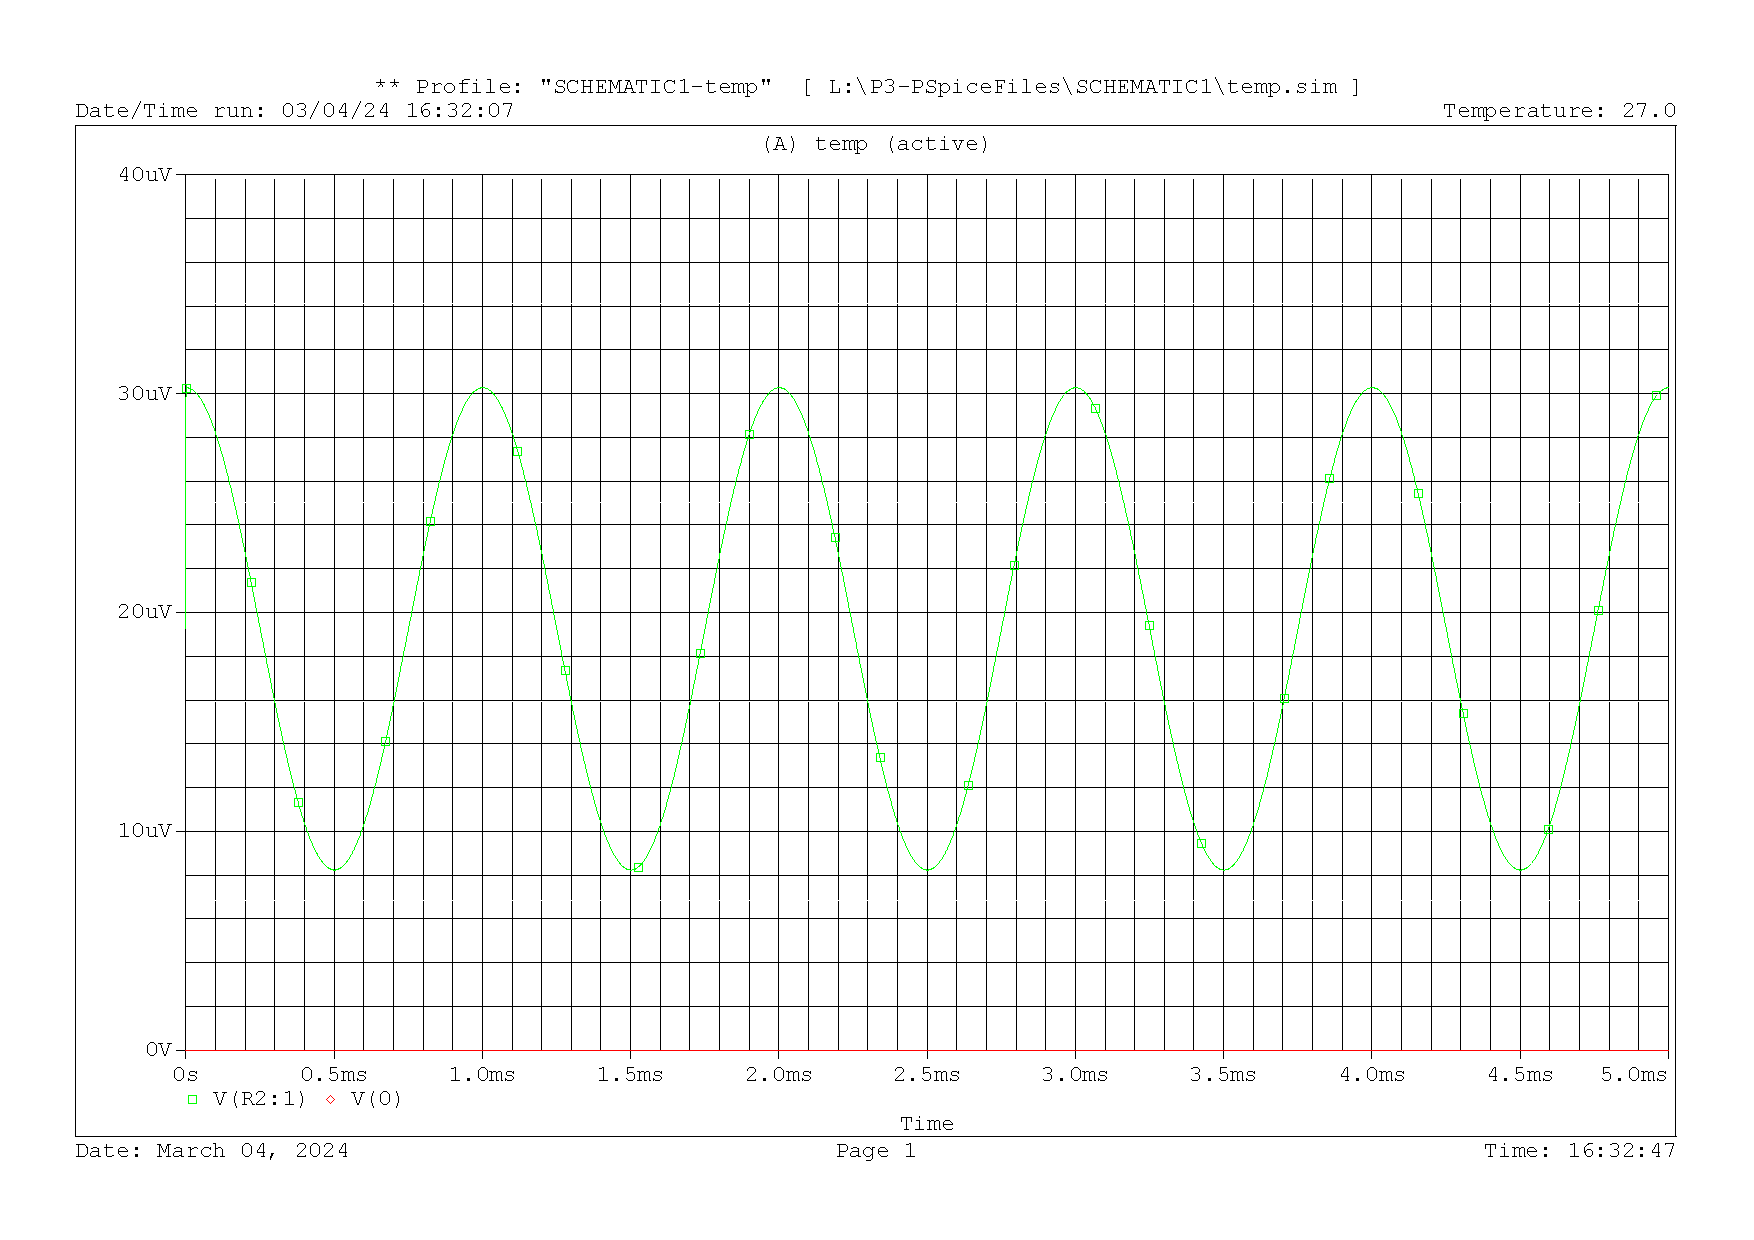
\includegraphics[width=\linewidth]{q2.pdf}
    \end{center}
    \caption{Nodes inversor i no-inversor de l'amplificador}
    \label{fig:q2}
\end{figure}

\newthought{Qüestió 1.3} Veure la figura \ref{fig:q3}. L'amplada de banda del amplificador operacional és limitat. Amb un guany determinat és comporta com un filtre passabaixes amb una certa freqüència de tall. Això afecta tant al desfasament com a l'amplitud.
\begin{figure}[h]
    \begin{center}
        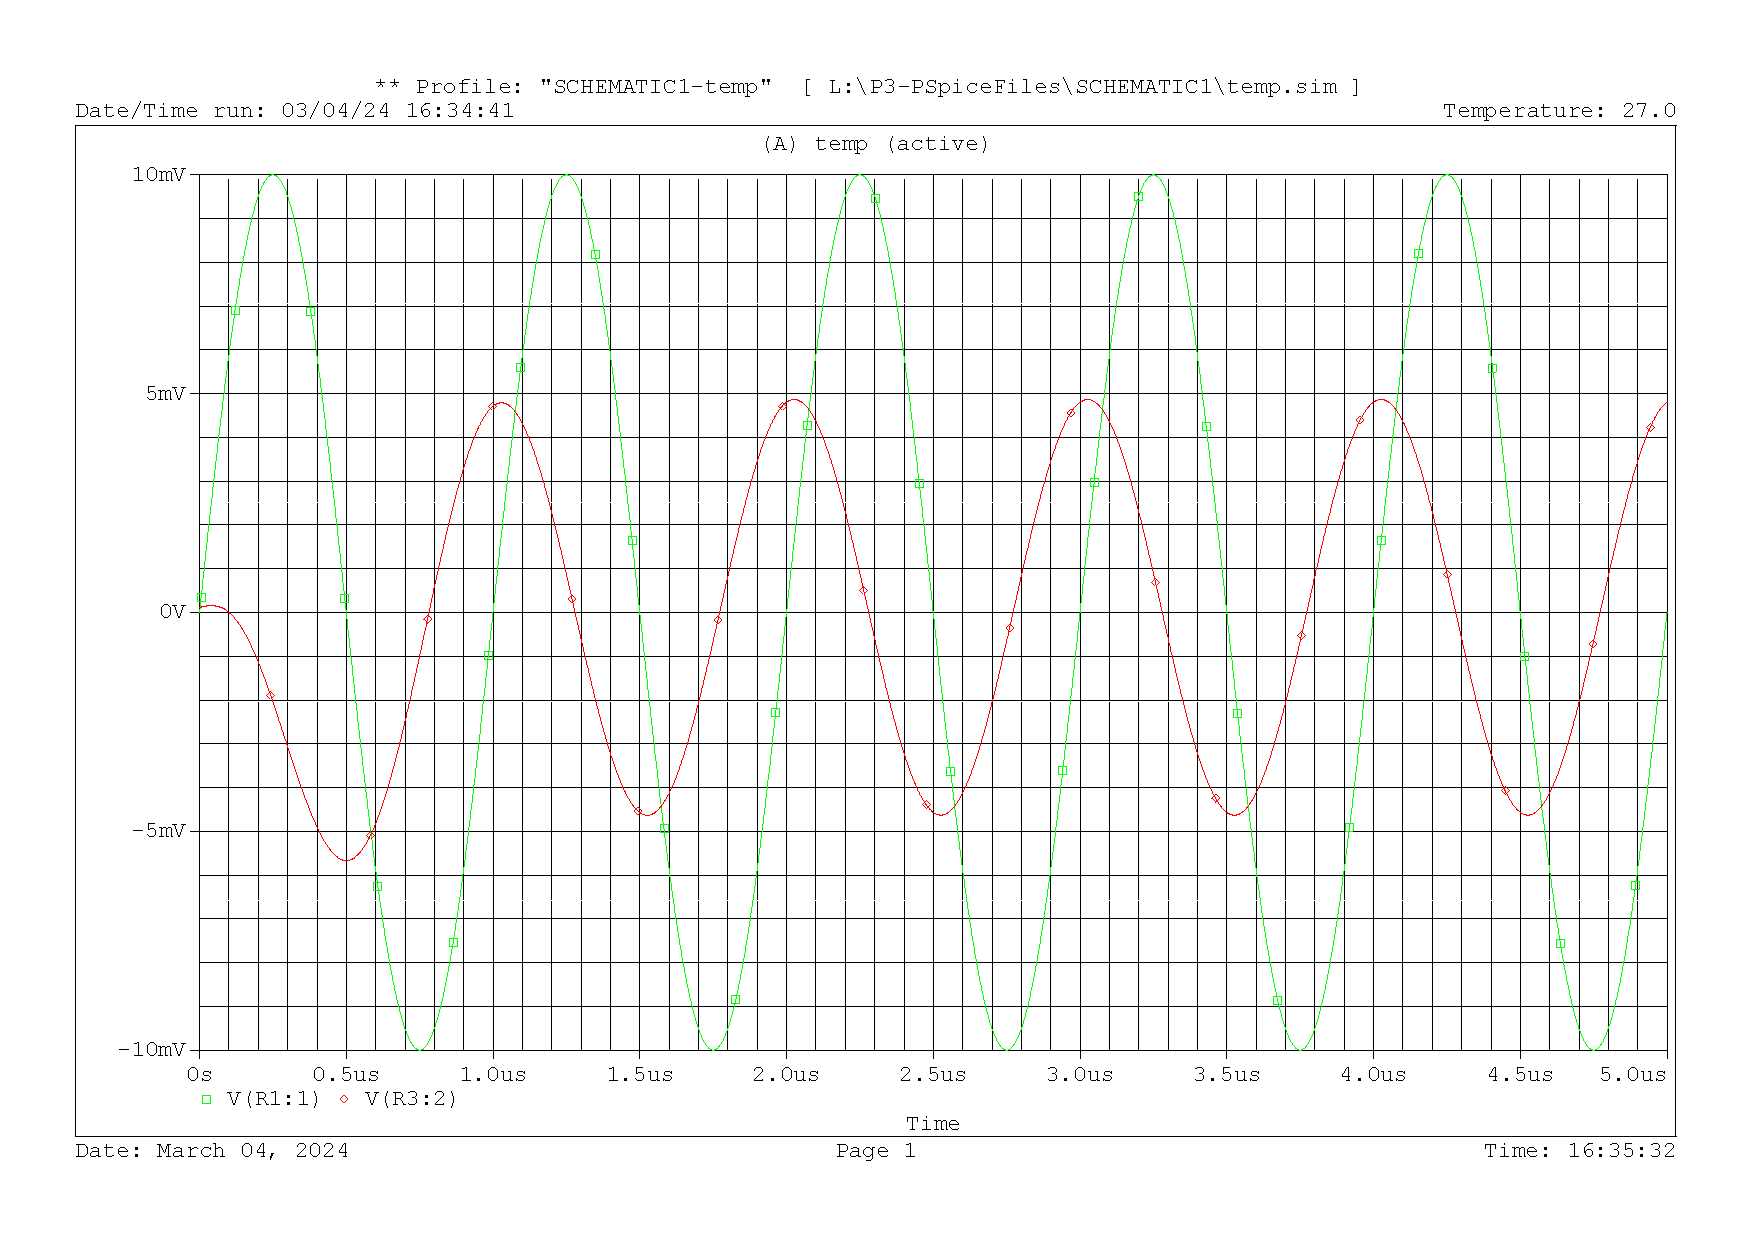
\includegraphics[width=\linewidth]{q3.pdf}
    \end{center}
    \caption{Entrada i sortida de l'inversor a \qty{1}{\mega\hertz}}
    \label{fig:q3}
\end{figure}

\section{2. Saturació de la tensió de sortida (marges dinàmics)}
\newthought{Qüestió 2.1} Veure la figura \ref{fig:q4}. El guany és $G=\qty{10}{\volt\per\volt}$ i el desfasament és \ang{180}.
\begin{figure}[h]
    \begin{center}
        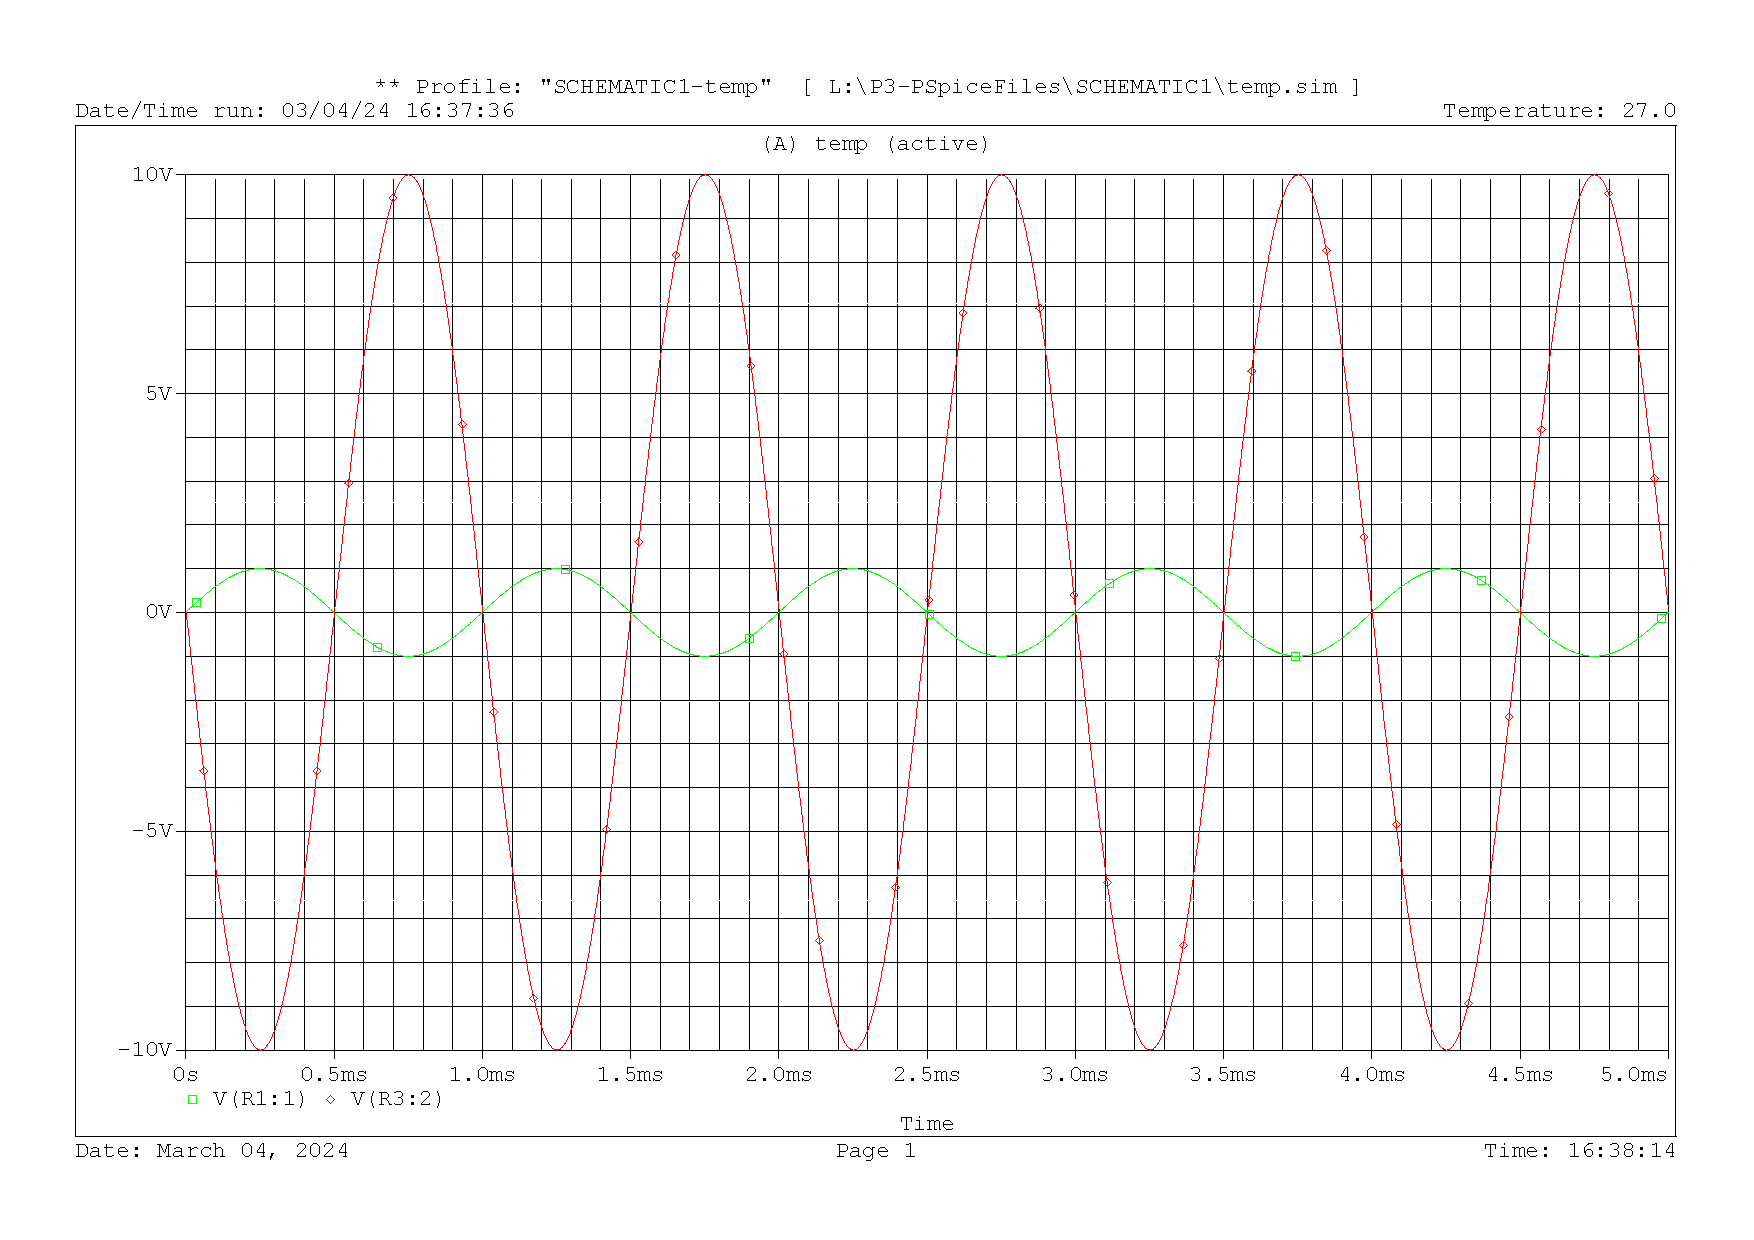
\includegraphics[width=\linewidth]{q4.pdf}
    \end{center}
    \caption{Entrada i sortida de l'inversor}
    \label{fig:q4}
\end{figure}

\newthought{Qüestió 2.2} Veure la figura \ref{fig:q5} (imatge inferior). S'observen deformacions a partir dels \qty{15}{\volt} a la sortida. Efectes de la saturació. La fase es conserva bé.

\newthought{Qüestió 2.3} Veure la figura \ref{fig:q5} (imatge superior). Quan es satura l'amplificador el node no-inversor arriva a tensions de gairebé \qty{500}{\milli\volt}. En aquestes condicions és impossible aplicar curtcircuit virtual.
\begin{figure}[h]
    \begin{center}
        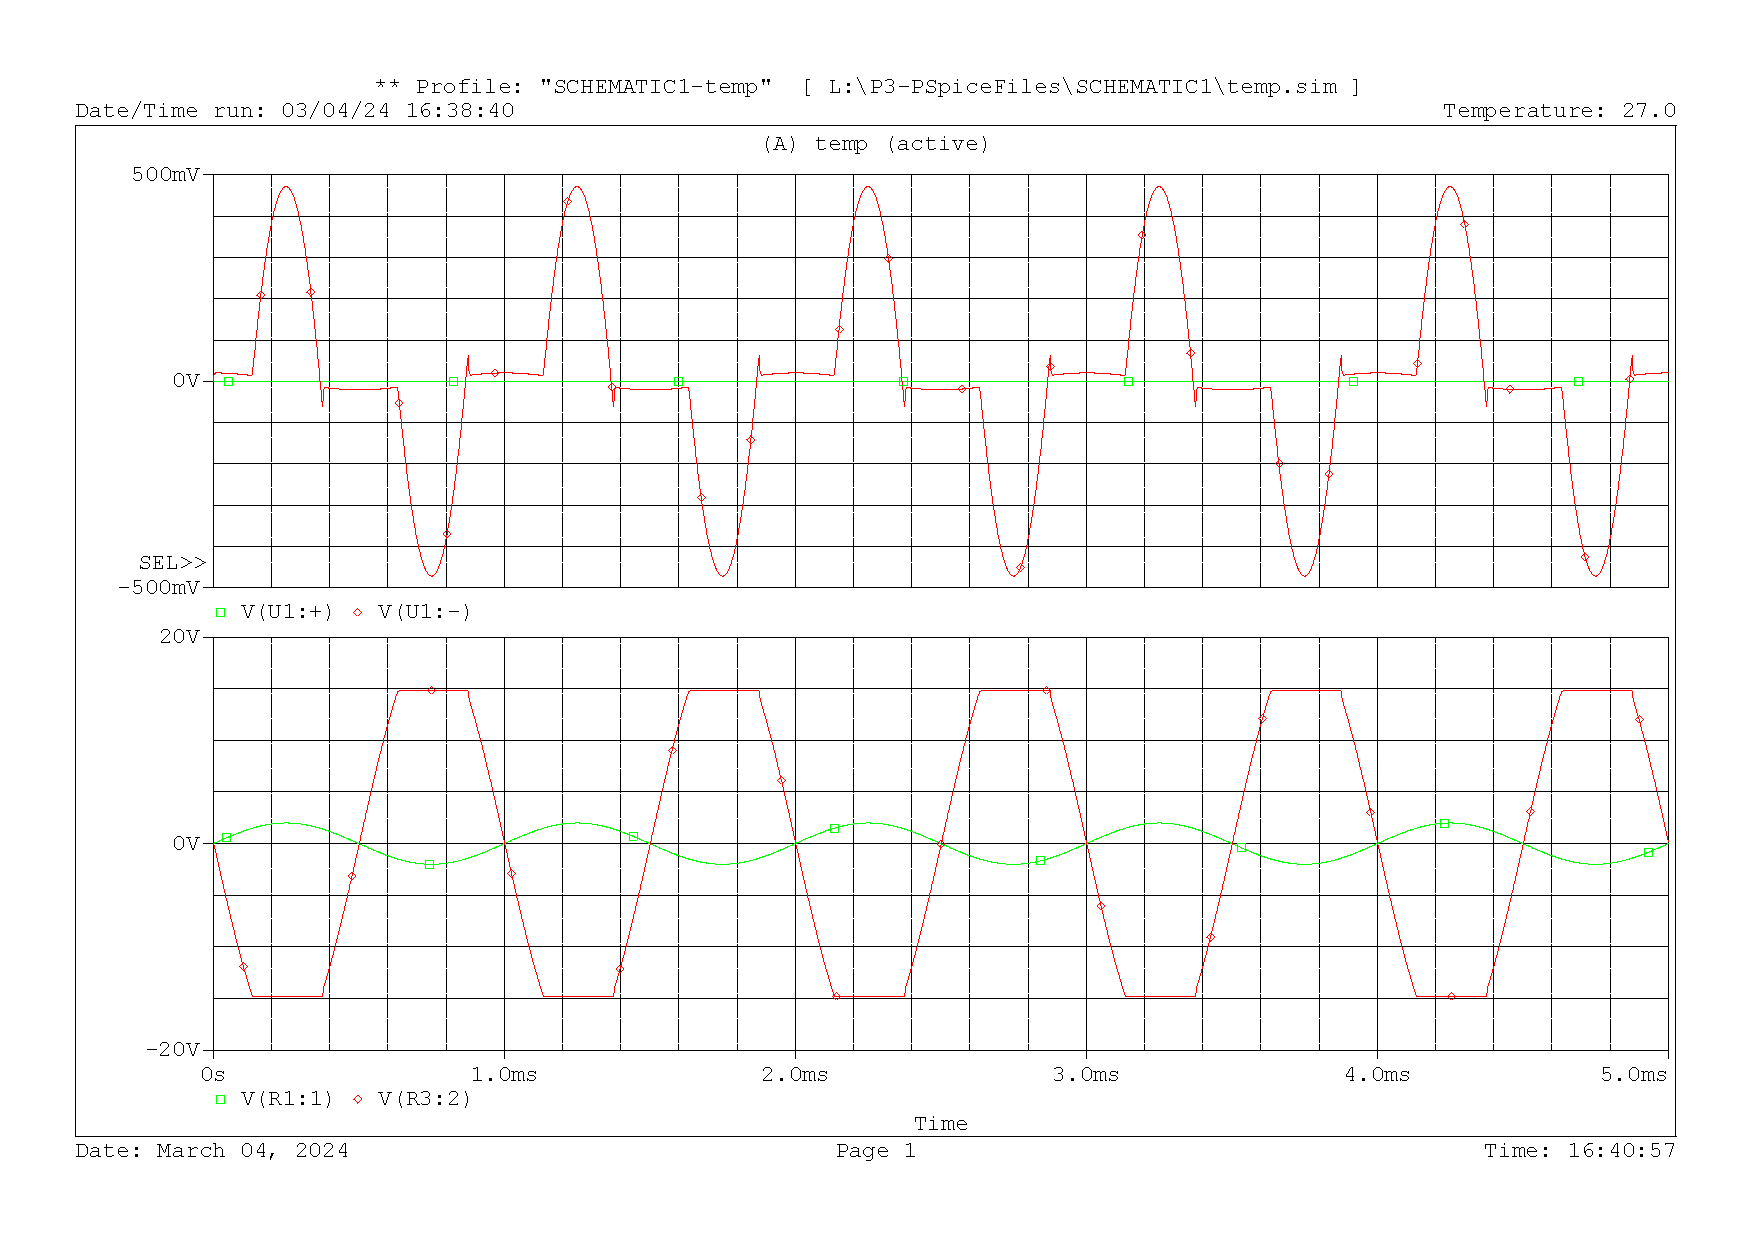
\includegraphics[width=\linewidth]{q5_2.pdf}
    \end{center}
    \caption{Entrada i sortida de l'inversor amb efectes de saturació}
    \label{fig:q5}
\end{figure}

\newthought{Qüestió 2.4} El llindar està al voltant dels $V_{max}=\frac{V_{cc}}{G}=\qty{1.5}{\volt}$. Tot i que el llindar real és una mica més baix. Es poden apreciar lleugerament no linealitats als pics de la simulació.

\section{3. Errors en contínua. Tensió d'offset i corrents de polarització}
\newthought{Qüestió 3.1} El senyal de sortida té una tensió d'offset d'uns $\simeq\qty{100}{\micro\volt}$. Això es degut a la tensió d'offset del amplificador operacional. Normalment no seria apreciable, pero amb senyals d'amplitud tan petita es pot veure el seu efecte.

\newthought{Qüestió 3.2} La sortida té un valor constant de $\simeq\qty{120}{\micro\volt}$.

\newthought{Qüestió 3.3} Ara la sortida té un valor constant de $\simeq\qty{1}{\milli\volt}$.

\newthought{Qüestió 3.4} La tensió de sortida té un valor de $\simeq\qty{850}{\micro\volt}$.

\newthought{Qüestió 3.5} No és només la tensió d'offset el que causa errors de contínua. La tensió que cau a les resistències a causa de les corrents de polarització també s'amplifica i té un impacte a la sortida. Per aquest motiu en cambiar els valors de les resistències em vist variacions que no poden ser només fruit de una tensió offset amplificada.

\newthought{Qüestió 3.6} La tensió de sortida té un valor de $\simeq\qty{40}{\micro\volt}$. La tensió que cau en la resitència que acabem de posar s'amplifica de manera no inversora i compensa l'error anterior. També és important veure que el valor de la resistència és el para\l.lel de les resistències del amplificador no inversor. És el valor òptim per anu\l.lar l'error.

\newthought{Qüestió 3.7} A partir de les primeres dues mesures s'obté

\begin{align}
    2 v_{off} + 10^3 i_n &= 120 \cdot 10^{-6} \\
    11 v_{off} + 10^4 i_n &= 1 \cdot 10^{-3}
\end{align}

D'on podem extreure que $v_{off} \simeq \qty{22.23}{\micro\volt}$ i $i_n \simeq \qty{75.56}{\nano\ampere}$. Amb la tercera mesura sabem que és certa l'equació

\begin{equation}
    2 v_{off} + 10^4 i_n - 10^4 i_p = 40 \cdot 10^{-6}
\end{equation}

D'on podem extreure que $i_p \simeq \qty{76}{\nano\ampere}$.

\section{4. Error en mode comú}
\newthought{Qüestió 4.1} El senyal hauria de ser cuadrat de \qty{2}{\milli\volt} pic a pic.

\newthought{Qüestió 4.2} El senyal està sumat a un sinus. No és el previst.

\newthought{Qüestió 4.3} El guany diferencial és \qty{1}{\volt\per\volt}.

\newthought{Qüestió 4.4} El guany comú és \qty{-0.01}{\volt\per\volt}.

\part{Segona sessió}
\section{5. Resposta freqüencial}
\newthought{Qüestió 5.1} Un desfasament de \ang{180} i un guany de \qty{0}{\deci\bel}.

\newthought{Qüestió 5.2} Una amplada de \qty{650}{\kilo\hertz}.

\begin{figure}[h]
    \begin{center}
        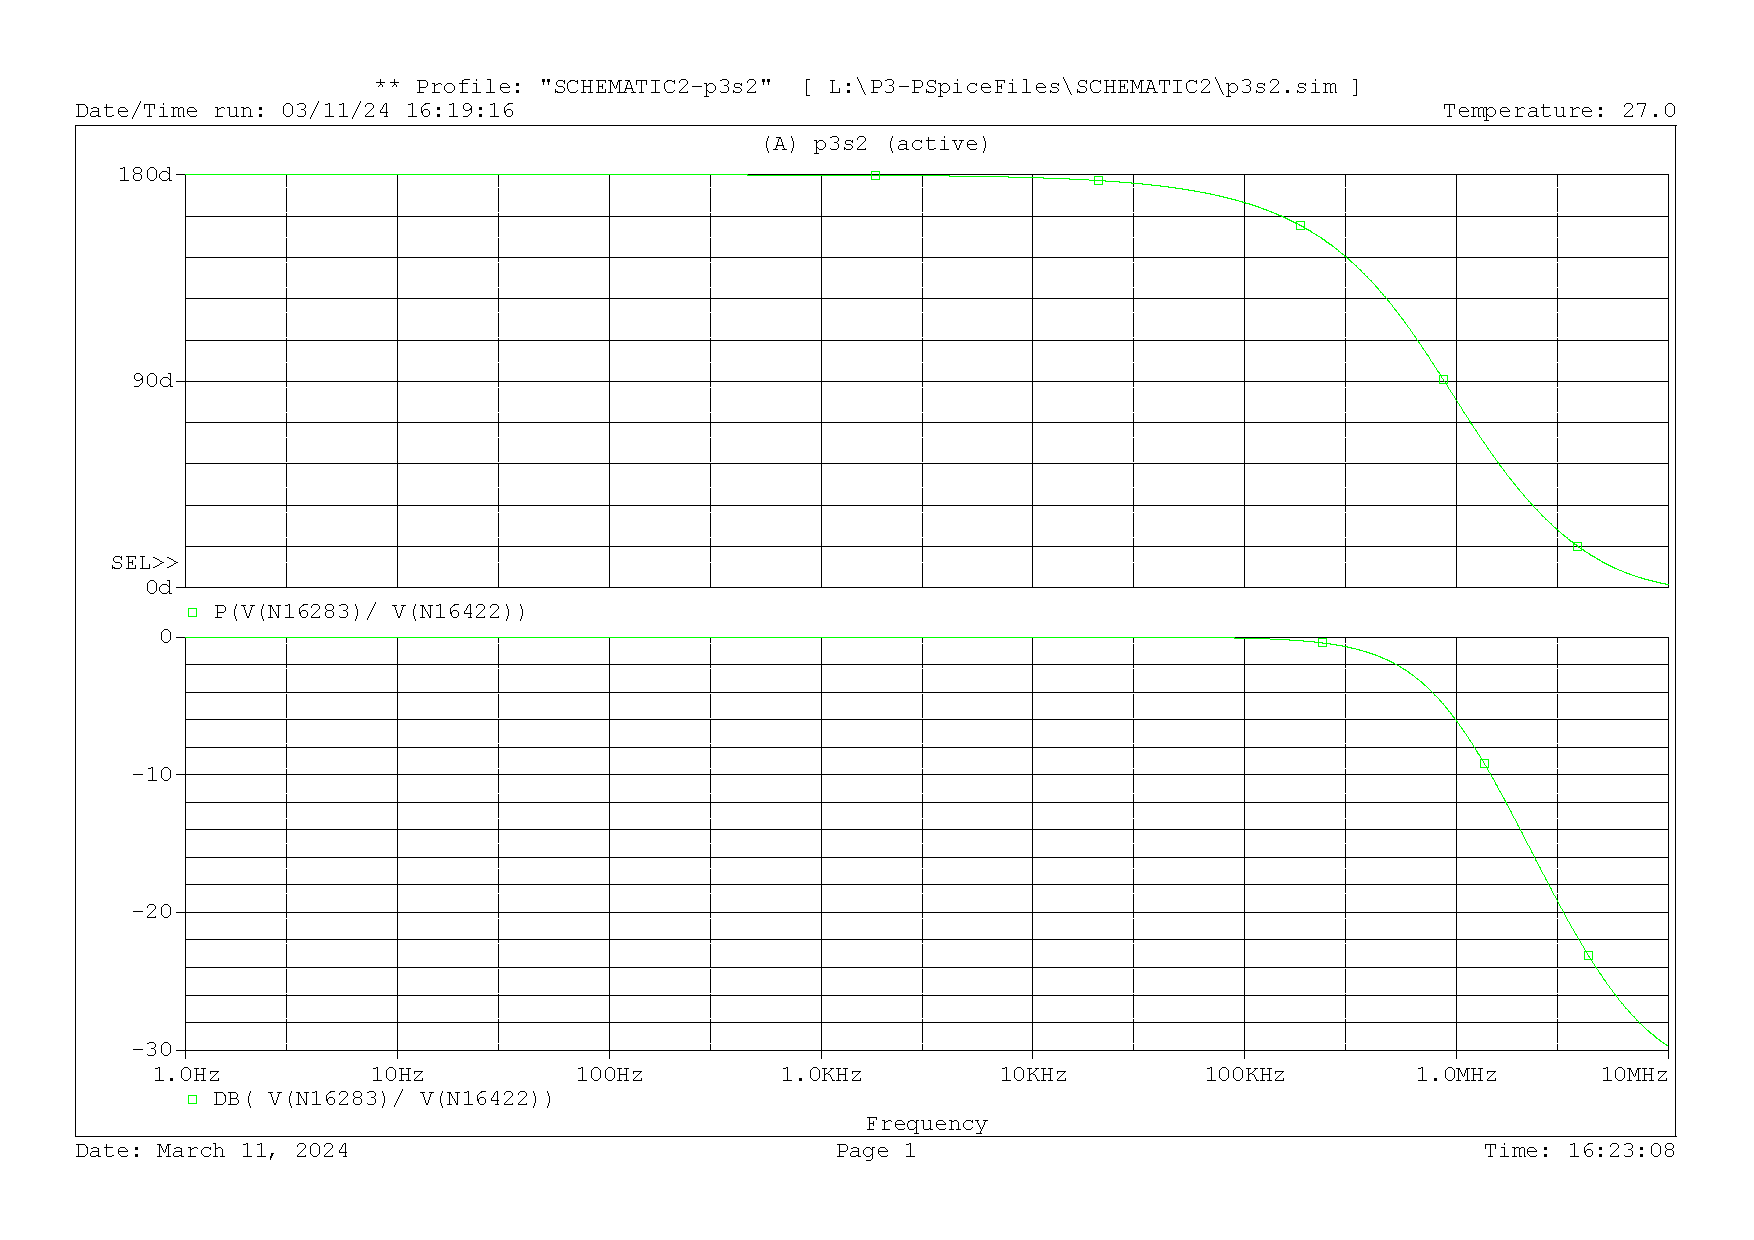
\includegraphics[width=300px]{s2/5_1.pdf}
    \end{center}
    \caption{Diagrama de Bode del inversor}
    %\label
\end{figure}

\section{6. Producte Guany-Ample de Banda (compromís entre guany i ample de banda)}
\newthought{Qüestió 6.1} El producte Guany-Ample de banda és constant.

\begin{table}
    \begin{center}
      \begin{tabular}{@{}rccc@{}}
        \toprule
        Resistència & \qty{1}{\kilo\ohm} & \qty{10}{\kilo\ohm} & \qty{100}{\kilo\ohm} \\
        \midrule
        Guany & \qty{0}{\deci\bel} & \qty{20}{\deci\bel} & \qty{40}{\deci\bel} \\
        \midrule
        Amplada de banda & \qty{650}{\kilo\hertz} & \qty{65}{\kilo\hertz} & \qty{6.5}{\kilo\hertz} \\
        \bottomrule
      \end{tabular}
    \end{center}
    \caption{Guany i amplada de banda per cada resistència}
    \label{tab:t1}
\end{table}

\begin{figure}[h]
    \begin{center}
        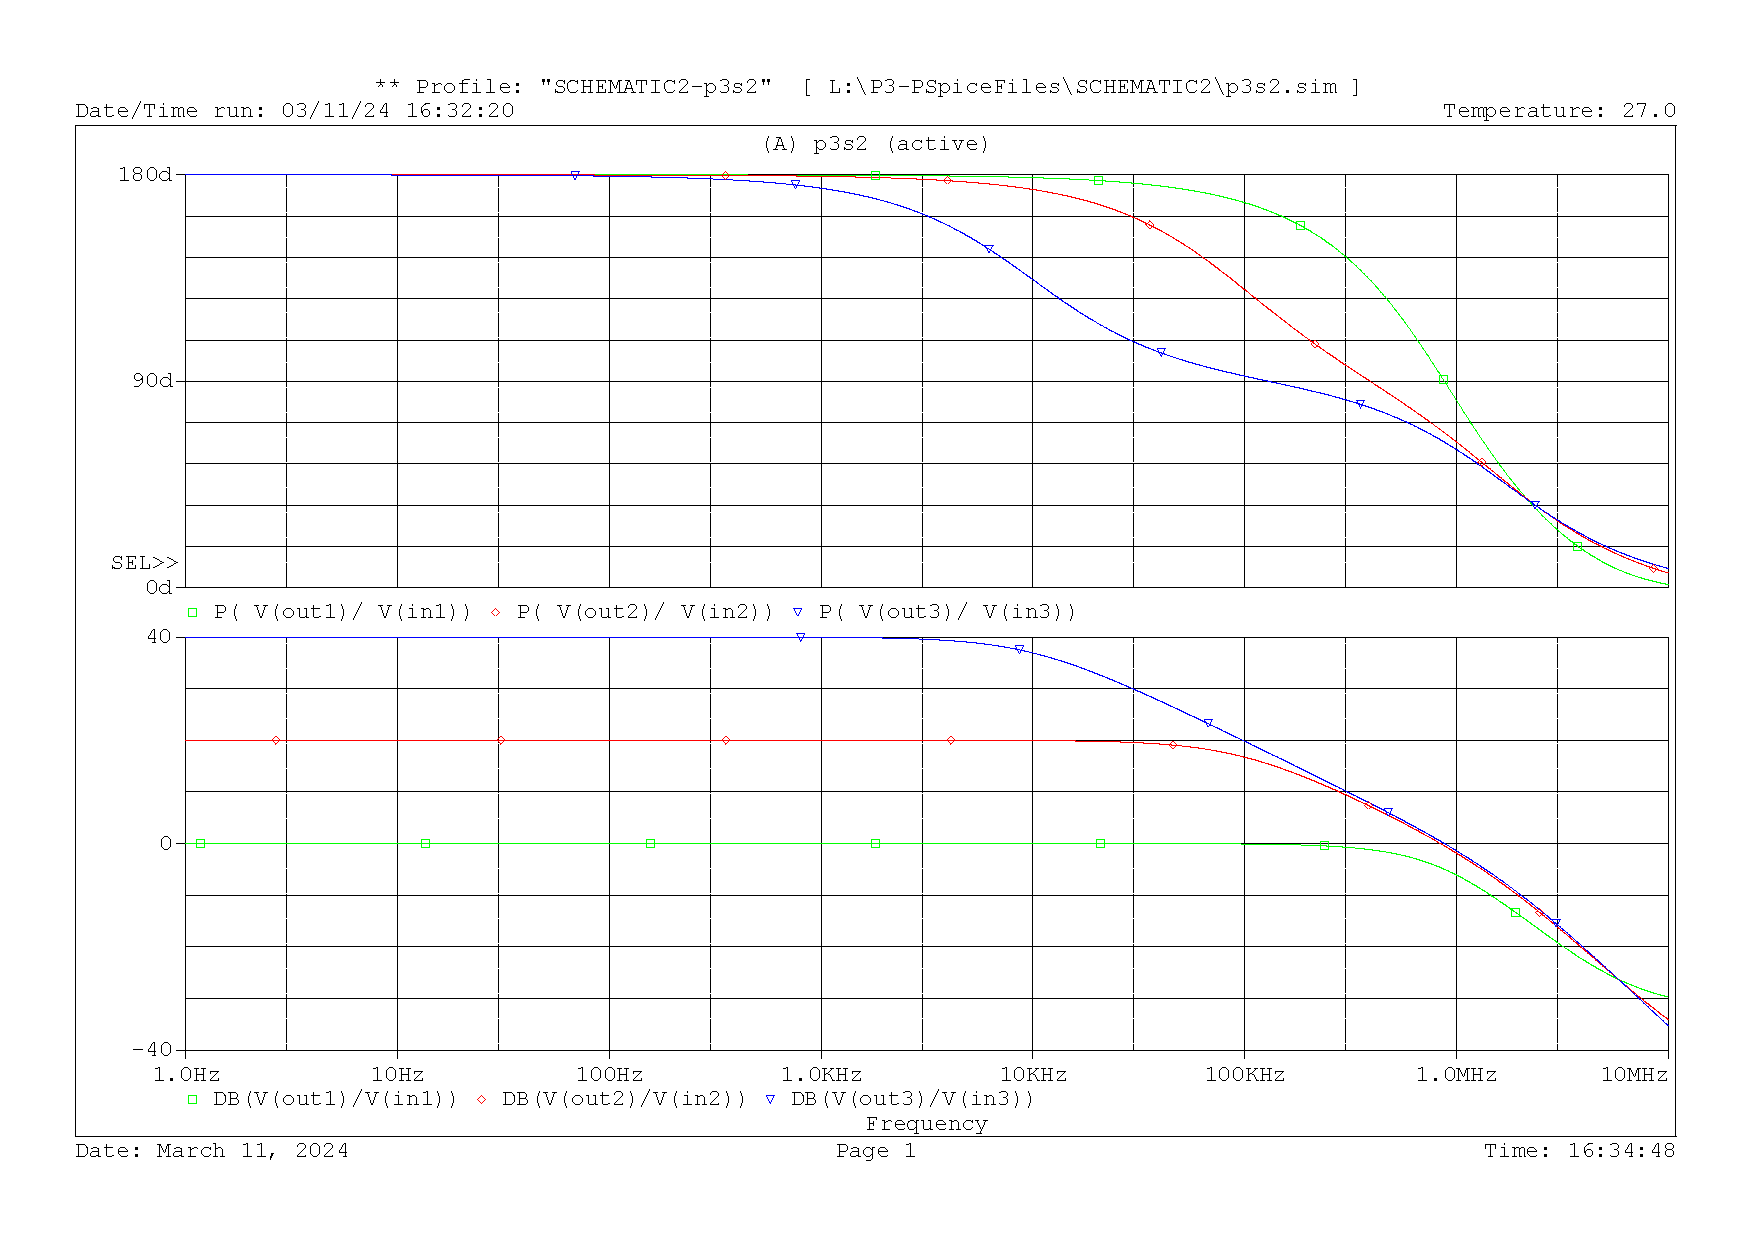
\includegraphics[width=300px]{s2/6_1.pdf}
    \end{center}
    \caption{Diagrama de Bode del inversor per diferents valors de resistència}
    %\label
\end{figure}

\newthought{Qüestió 6.2} La freqüència de guany unitari és $f_t = \qty{875}{\kilo\hertz}$.

\newthought{Qüestió 6.3} La tensió de sortida tindria efectes de saturació. El simulador ignora aquest efecte quan fa un sweep AC.

\section{7. Temps de Pujada}
\newthought{Qüestió 7.1} El temps de pujada és \qty{300}{\nano\second}. Es pot comprovar a la figura \ref{fig:q7}.

\begin{figure}[h]
    \begin{center}
        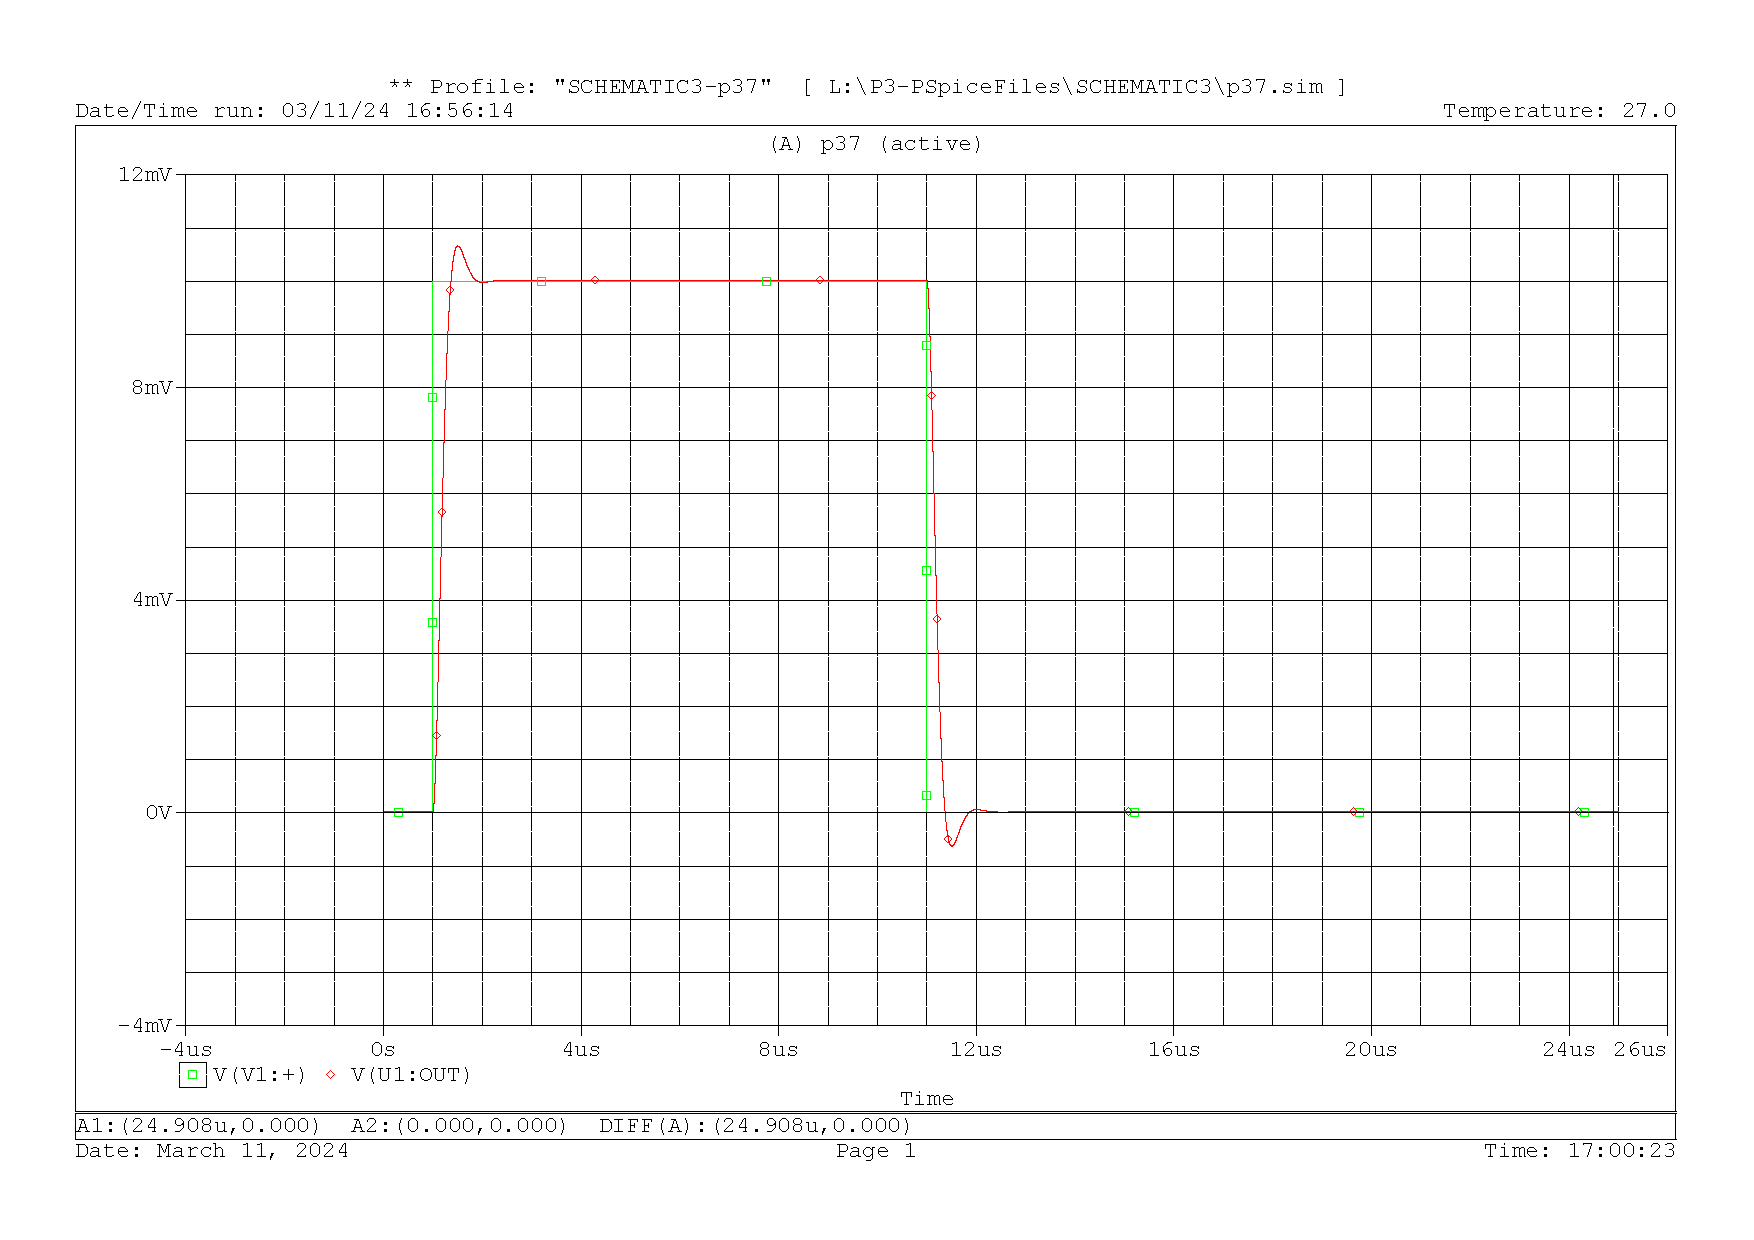
\includegraphics[width=300px]{s2/7_1.pdf}
    \end{center}
    \caption{Simulació temporal d'un pols rectangular}
    \label{fig:q7}
\end{figure}

\section{8. Slew-Rate}
\newthought{Qüestió 8.1} El overshoot que s'observa a la figura \ref{fig:q7} es causa de l'efecte passabaixes que te l'AO. En canvi, a la figura \ref{fig:q8_1} l'efecte predominant es el slew-rate, la incapacitat de produir una pendent tan gran com la desitjada. La máxima pendent és \qty{0.5}{\volt\per\micro\second}. La mesura es correspon perfectament amb les especificacions.

\begin{figure}[h]
    \begin{center}
        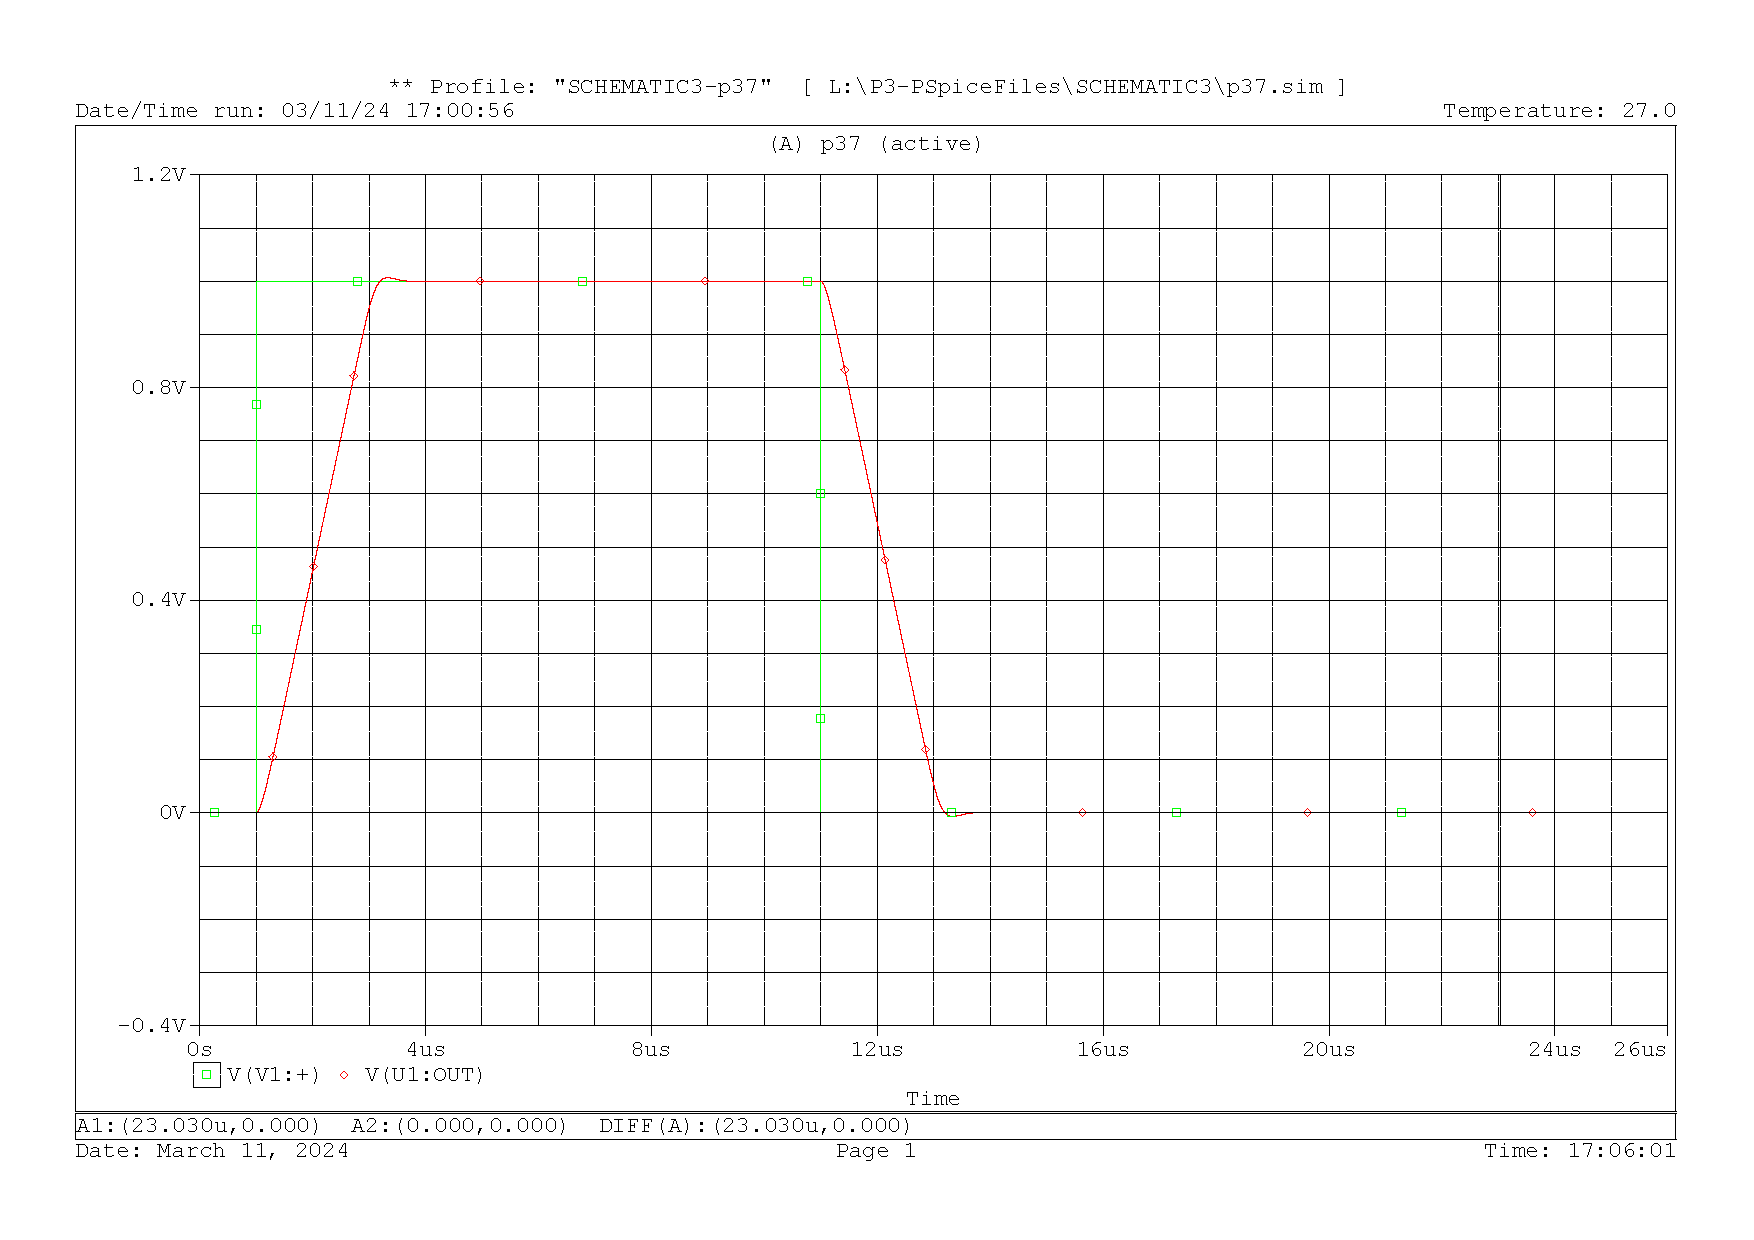
\includegraphics[width=300px]{s2/8_1.pdf}
    \end{center}
    \caption{Simulació temporal d'un pols rectangular de gran amplitud}
    \label{fig:q8_1}
\end{figure}

\newthought{Qüestió 8.2} El pendent màxim del senyal d'entrada correspon a \qty{0.032}{\volt\per\micro\second} que està molt per sota del slew-rate. No s'aprecia cap distorsió.

\newthought{Qüestió 8.3} Tenen pràcticament la mateixa FFT. Veure la figura \ref{fig:q8_3}.

\begin{figure}[h]
    \begin{center}
        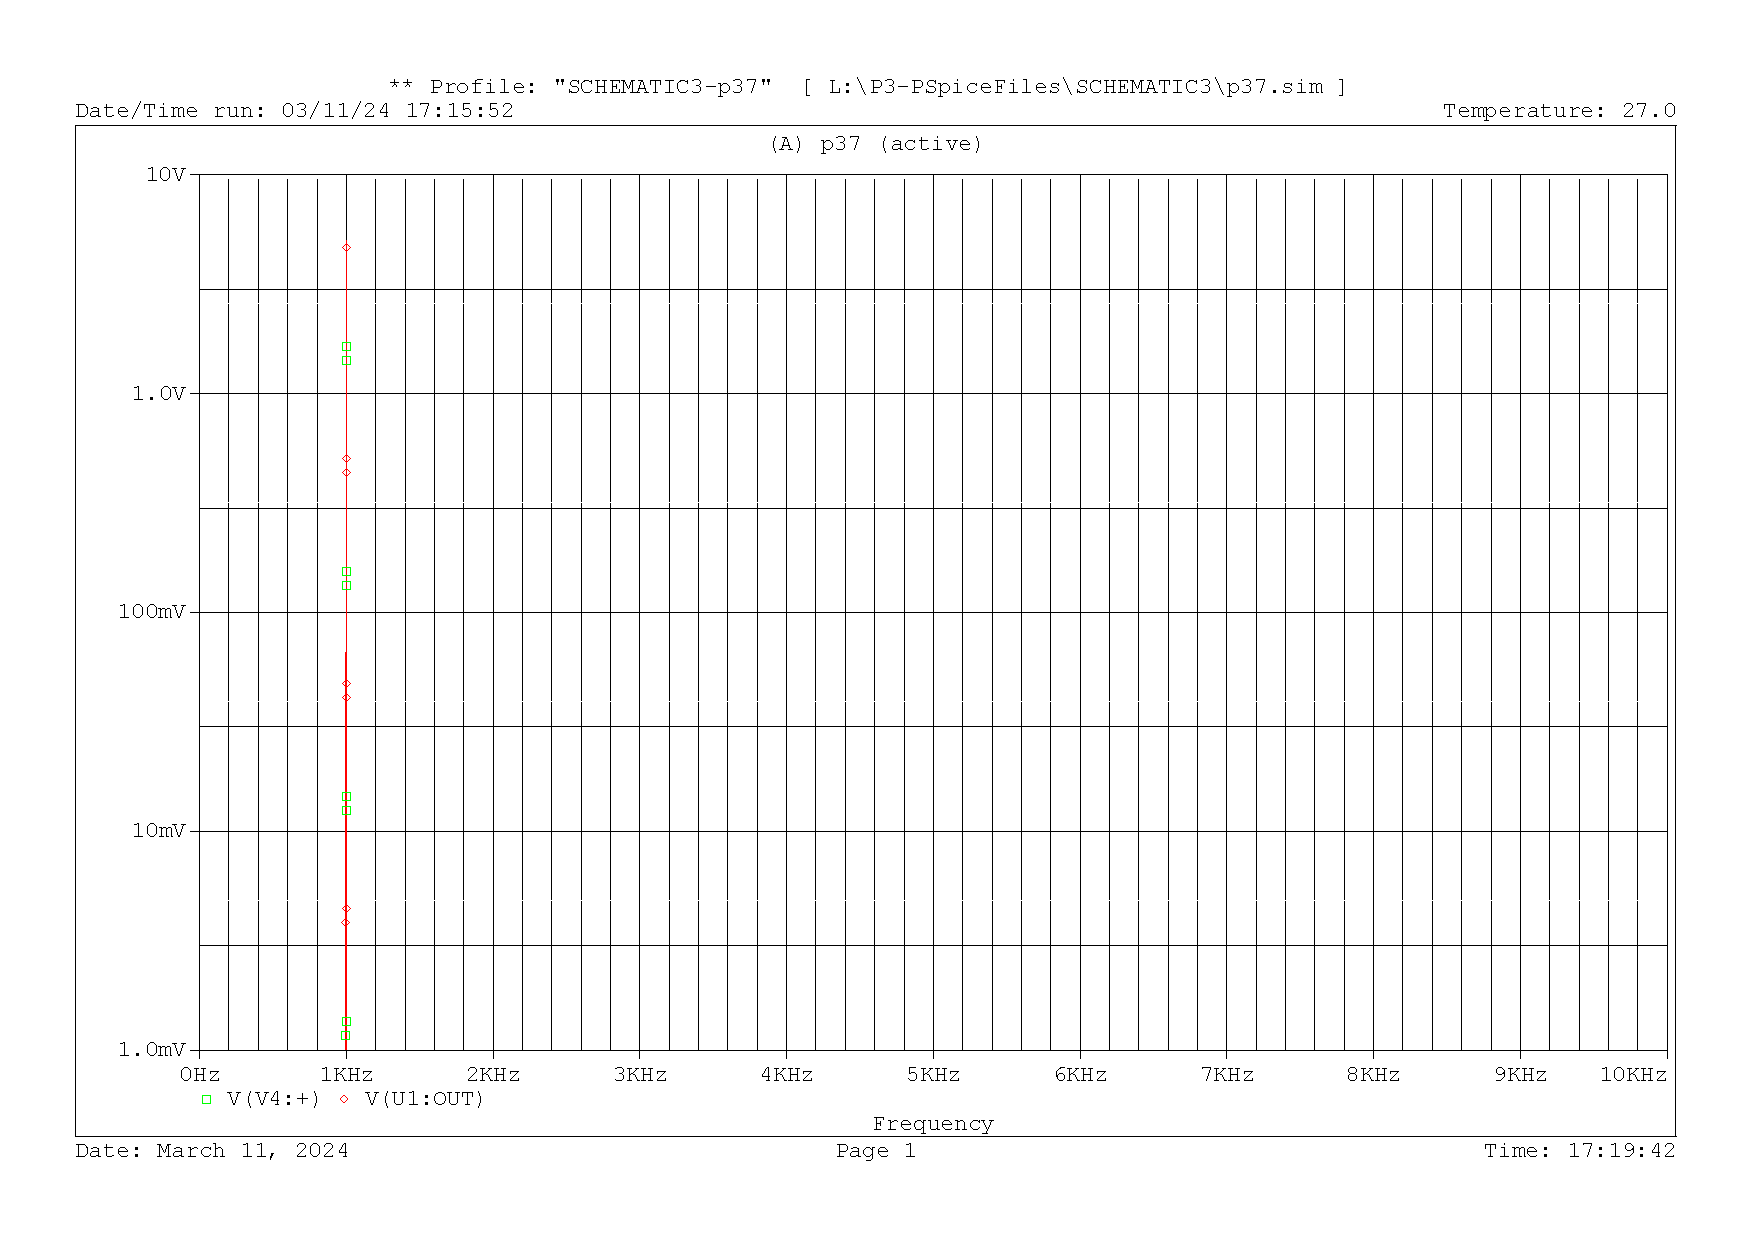
\includegraphics[width=300px]{s2/8_2.pdf}
    \end{center}
    \caption{FFT de l'entrada i sortida}
    \label{fig:q8_3}
\end{figure}

\newthought{Qüestió 8.4} Es pot apreciar distorsió. Veure la figura \ref{fig:q8_4}

\begin{figure}[h]
    \begin{center}
        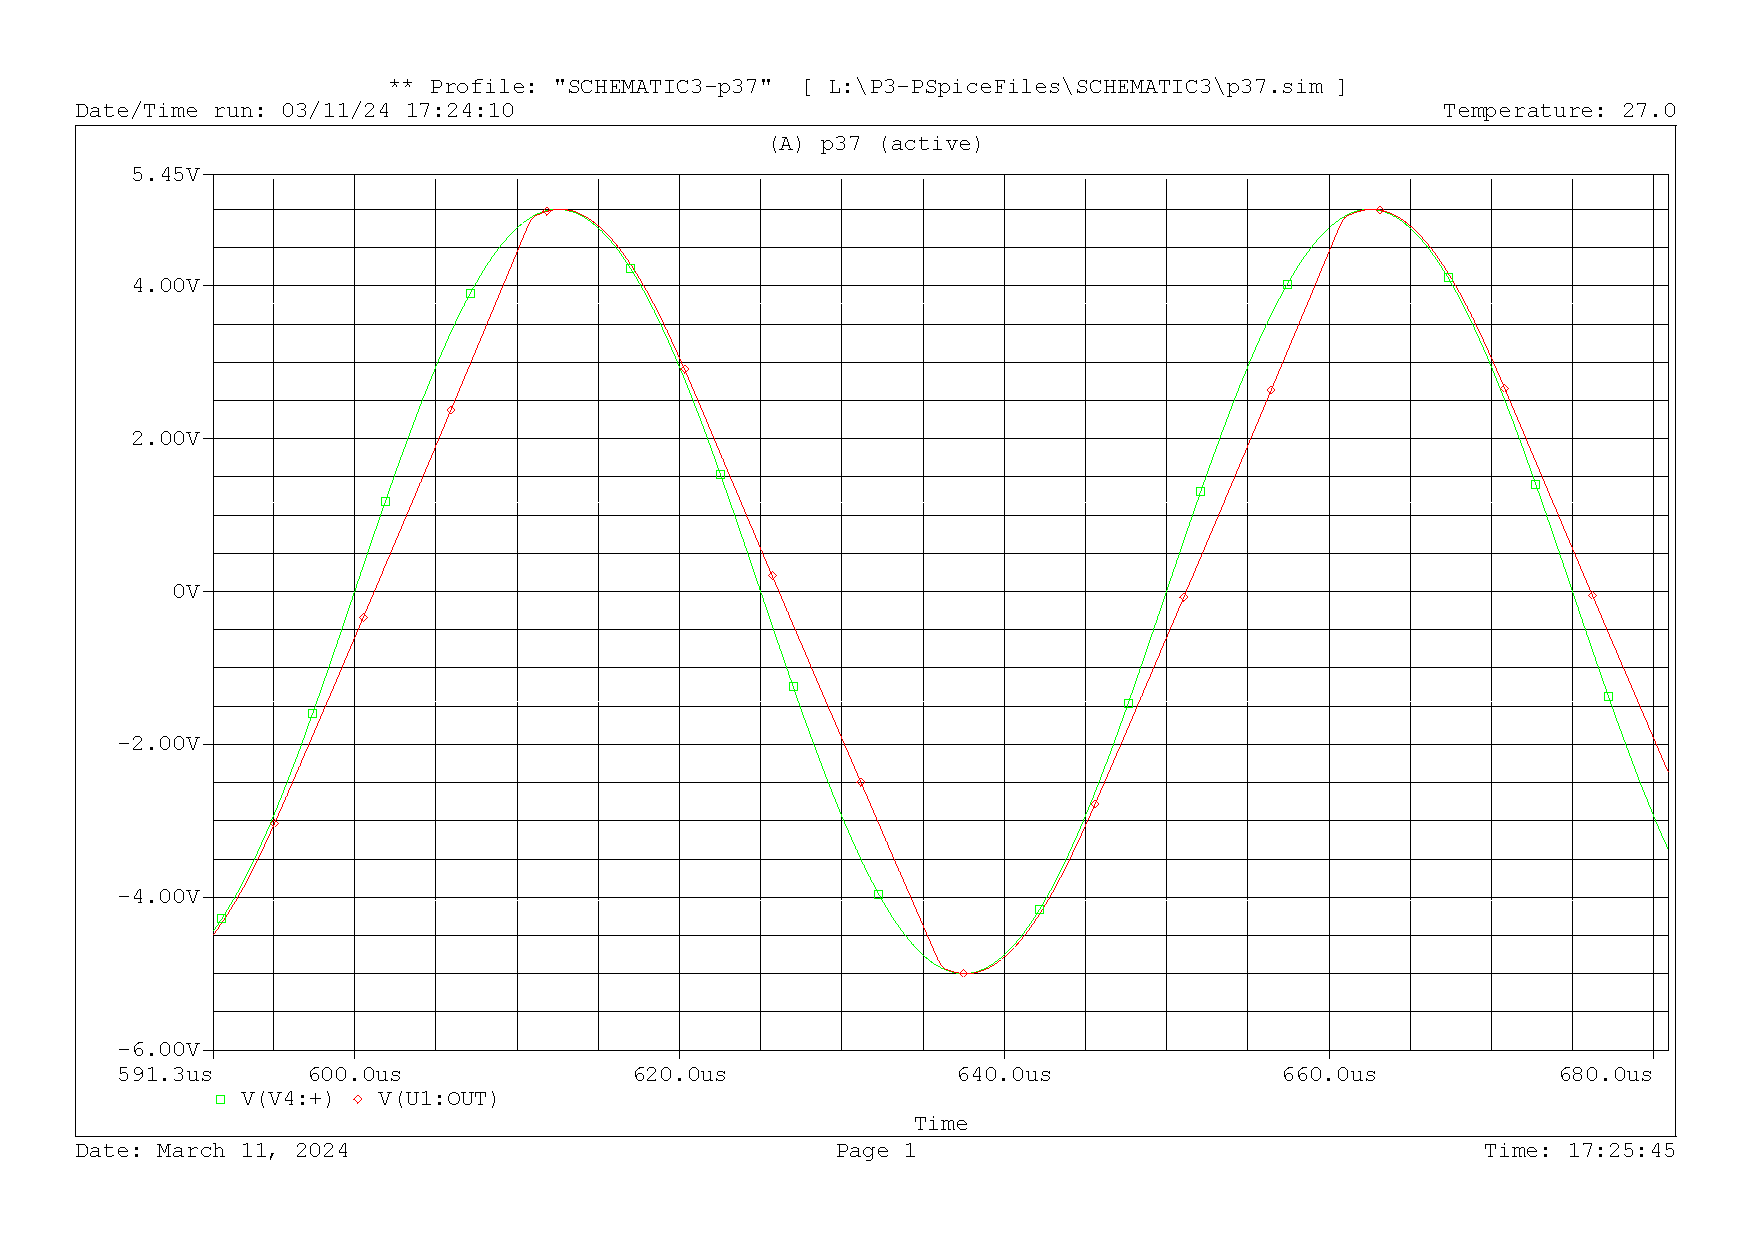
\includegraphics[width=300px]{s2/8_3_2.pdf}
    \end{center}
    \caption{Simulació temporal, efecte del slew-rate sobre un sinus}
    \label{fig:q8_4}
\end{figure}

\newthought{Qüestió 8.5} Els efectes no lineals sobre senyals periòdics suposen nou contingut freqüencial als compoenens harmònics. Veure la figura \ref{fig:q8_5}.

\begin{figure}[h]
    \begin{center}
        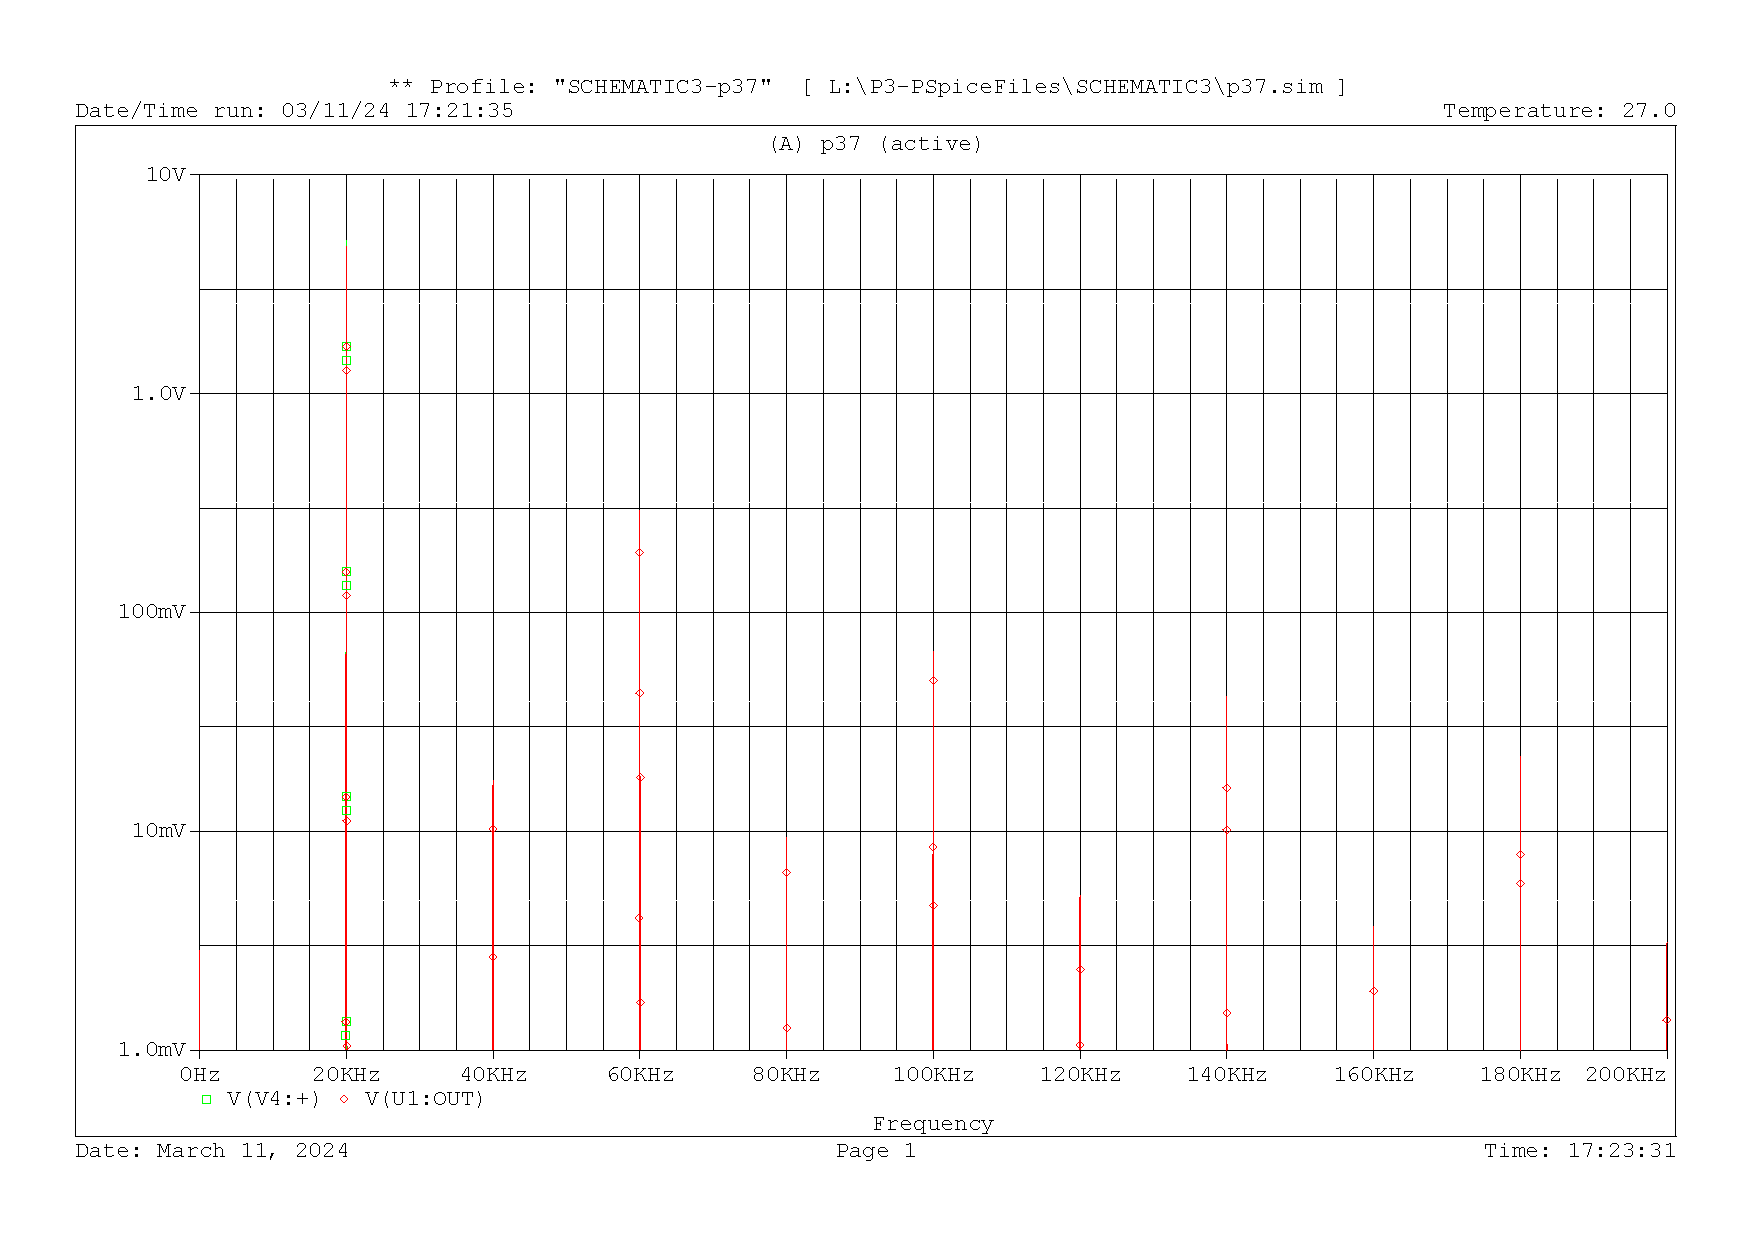
\includegraphics[width=300px]{s2/8_3.pdf}
    \end{center}
    \caption{FFT d'entrada i sortida}
    \label{fig:q8_5}
\end{figure}

\end{document}
